
\section{Defining e-waste}

E-waste, also known as \textit{Waste Electrical and Electronic Equipment} (WEEE), includes most electronics that requires an electric current or a battery to function \cite{WEEE}. In 2019 the global generation of e-waste was 53.6 million mt \cite{sanchez2024}, which is predicted to increase to 74.7 metric tons by 2030, which is not including solar panels \cite{javed2024}. Looking at only solar panels, it is predicted that they will contribute to 4-14\% of the e-waste in 2030 and over 50\% (~78 million tons) in 2050 \cite{javed2024}. The e-waste market is expected to grow to \$145 million by 2030 (src6 -> 3). Recovering REEs from e-waste is driven by environmental (avoiding new exploitation and having circular \textit{techonomy}), geopolitical (reducing dependency on single suppliers), and economical (reducing costs when traditional supply is dwindling and stabilizing global supply) factors \cite{sanchez2024}.

The world's leading countries for the generation of e-waste are China (10.1 million tons), the US (6.9 million tons), and India (3.2 million tons) \cite{javed2024}. One paper estimates that recycling Nd-Fe-B magnets from old hard drives in the US only, could supply 5.2\% of the global (excluding China) demand for those REEs (src6 -> 10).

The composition of e-waste is 65\% metals, 21\% plastics, 16\% other materials (\cite{javed2024} Take figure 6 from the paper). The metals are 50\% ferrous metals such as iron and steel, and 13\% non-ferrous metals such as copper, aluminium, precious metals, and rare-earth elements. 

1 million cell phones equal 35274 lbs of copper, 772 lbs of Ag, 75 lbs of Au, and 33 lbs of palladium \cite{javed2024}.

\section{Recycling and recovery}

The recovery of REEs from end-of-life (\textit{EOL}) products is a challenge that is gaining more attention as the demand for REEs increases \cite{USDoE2024}. Another reason for the increase in interest in recycling REEs is the environmental impact of mining and processing REEs \cite{REELandscape}. Presently it is mostly phosphors and catalysts that are recycled \cite{britannica2024}. However, batteries such as nickel-metal hydride (\textit{NiMH}) batteries and some permanent magnets hold 25-30\% of their weight in REEs, which is more than any ore deposit \cite{britannica2024}. Recycling aligns with a circular economy approach \cite{circular2016}, but recovery is difficult for many reasons, including the mixture of materials and metals in the products and the use of glass, polymers, and other non-metals.

Traditional methods involve using chemicals to dissolve the REEs from the product, and then precipitate them out of the solution \cite{sanchez2024}. Other methods also involve using heat or electricity to extract the REEs \cite{sanchez2024}. The similarities between the different extraction techniques are that they try to exploit the different chemical and physical properties of the REEs to separate them from each other and the ore or e-waste \cite{sanchez2024}. What makes this process difficult is that the REEs are chemically and physically similar to each other \cite{britannica2024}, which requires a high degree of precision and accuracy in the separation process.


\subsection{Hydrometallurgical recycling}

See src7 -> fig 10 for an overview of hydromeallurgical processes.

The hydrometallurgical process is a chemical process, where different chemicals, acids or bases, are used to leach, ie. dissovle, the REEs \cite{javed2024}. As seen in Figure \ref{fig:hydroprocess}, there are different categories of hydrometallurgical processes. The main three are chemical leaching, acid/alkali leaching, and bio-hydrometallurgical approach. Although the most used industrial process with a good recovery rate, its heavy use of chemicals comes with an environmental footprint.

\begin{figure*}
    \centering
    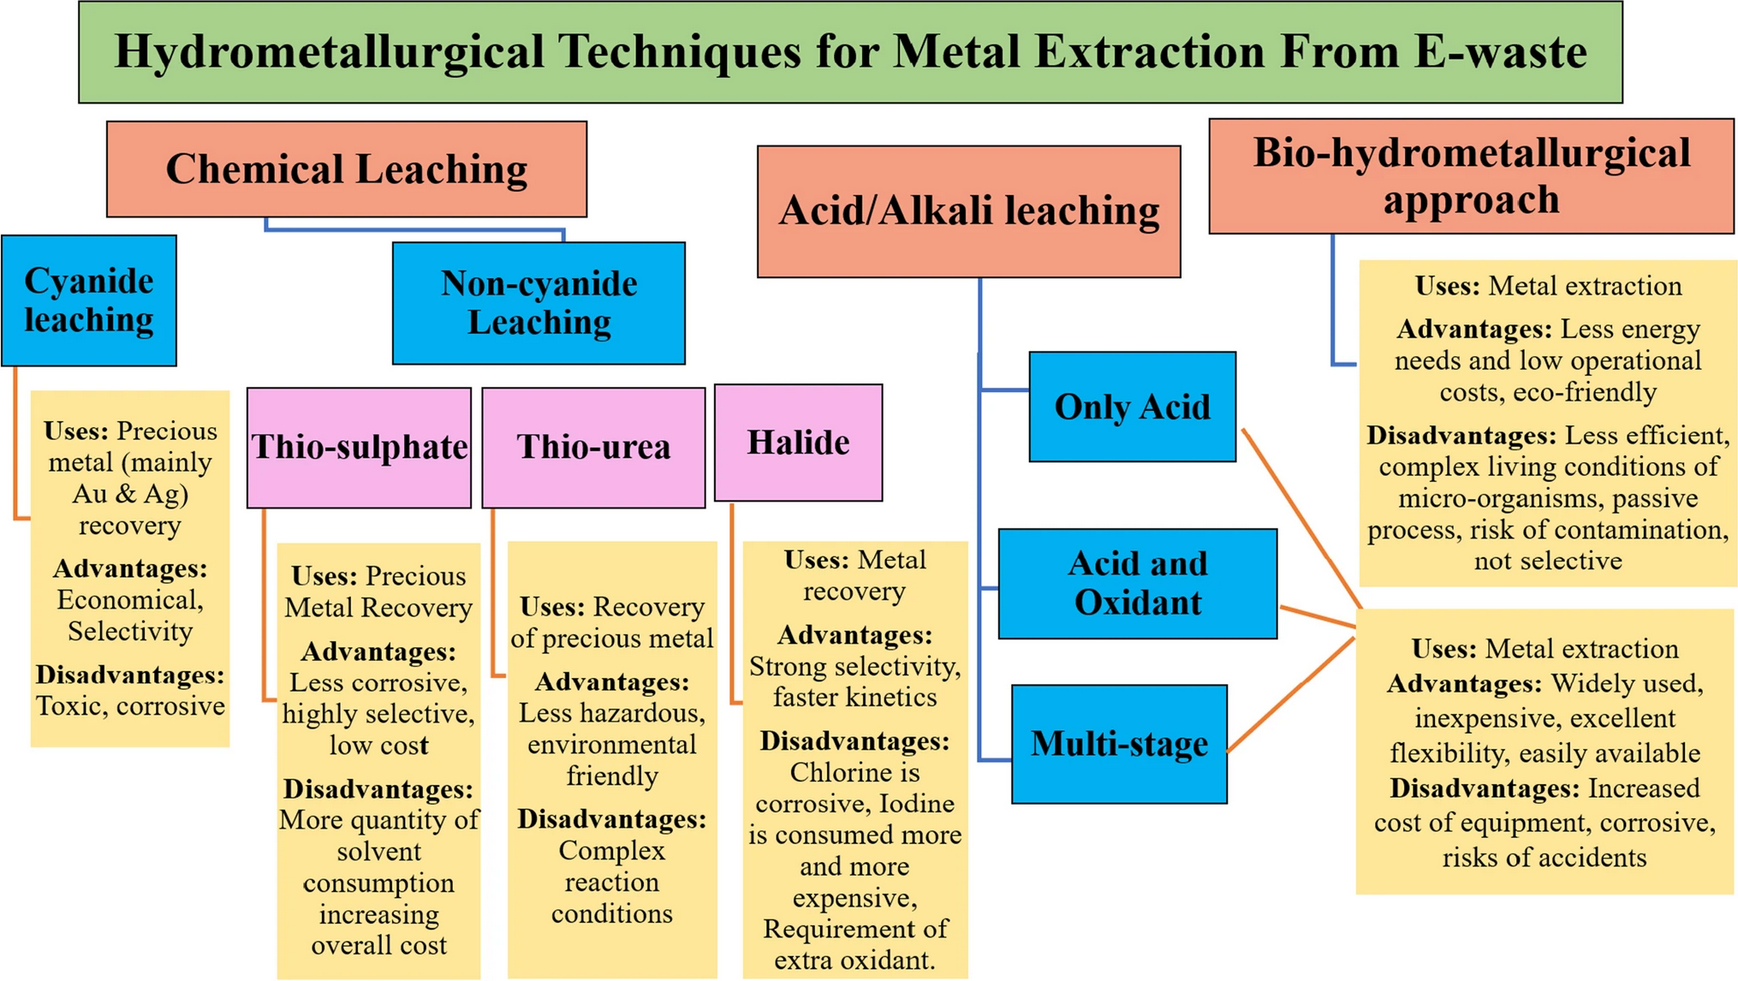
\includegraphics[width=1\linewidth]{figures/javier_processoverview.png}
    \caption{Overview of the different hydrometallurgical processes. Source \cite{javed2024}.}
    \label{fig:hydroprocess}
\end{figure*}

\subsubsection{Chemical leaching}

The four sub-categories of chemical leaching are \textit{cyanide leaching}, \textit{thio-sulphate leaching}, \textit{thei-urea leaching}, and \textit{halide leaching} \cite{javed2024}. The latter three can all be grouped as \textit{non-cyanide leaching}. As can be expected, the major drawback of cyanide leaching is that it is highly toxic and also highly corrosive (add src). The reason for using cyanide is that it is cheap to use and effective at extracting Au and Ag (src 7).

The non-cyanide group all have the advantages that they are less toxic than cyanide (add src), less corrosive (except halide), and theio-urea is also classified as environmentally friendly (add src). Which one to choose depends on which metal there is to be extracted (add src), even though they all are mostly used to extract precious metals (add src). Thiosulfate leaching has the issue that it is not as effective as cyanide, with about 93\% leaching rate for Au, and is also more expensive \cite{javed2024}. Thiourea leaching has a 99\% leaching rate for Au and works faster \cite{javed2024}. Halide leaching includes \textit{chloride}, \textit{bromide}, and \textit{iodide} leaching, and has an Au leaching rate of around 90\% \cite{javed2024}.

\subsubsection{Acid/alkali leaching}

Acid leaching is the most common approach for metal recovery from electronic waste \cite{javed2024}. The process is well-studied, flexible, and inexpensive. Different acids are used depending on which metal is to be recovered. Within acid leaching, there are three different approaches: acid only, acid and oxidiser agent, or multi-stage acid leaching. Depending on the method used and the metal type, the recovery rate is between 6-90%. 

\subsubsection{Bio-hydrometallurgical approach}

The use of bacteria or fungi is gaining attention as an alternative to traditional hydro- and pyrometallurgical methods \cite{javed2024}. In one study it was found that the bacteria \textit{Pseudomonas chlororaphis} was able to dissolve Ag, Au, and Cu at rates of 8.2\%, 12.1\%, and 52.3\% respectively \cite{bioleaching}. 

Another study looked at the fungi \textit{A. niger}, also known as \textit{black mold}, and found that in a two-step chemo-bioleaching process, a recovery rate of 70.6\% of Cu was achieved \cite{ANiger}. The use of biological agents is still new, and many variables have to be controlled to make the process reliable (pH, temperature, contamination, etc.) \cite{javed2024}. 

Ionic liquids (\textit{Ils}) can potentially play a role in the future of metal extraction \cite{javed2024}. Ils are often hydrophobic and can therefore also extract other hydrophobic materials. They do however come with the downside of being toxic and having poor biodegradability. Another future candidate is deep eutectic solvents (\textit{DES}), which overcome these problems of Ils \cite{javed2024}. 

Another compound that has been explored is glycine \cite{glycine}. It has shown to be effective at dissolving Cu at a rate of 98\% after 48 h. However, it does struggle with solving other metals such as Au and Ag \cite{javed2024}.

Chelating, which is the chemical process of binding a metal ion to a chemical compound, has also gained popularity in recent years \cite{javed2024}. By using biodegradable chemicals such as \textit{DTPA} or \textit{NTA}, metals such as Cr, Cu, Zn, and Pb can be removed from polluted soils \cite{javed2024}.

\subsection{Pyrometallurgical recycling}

Also called \textit{thermal extraction}, pyrometallurgy is a method that uses high heat to extract materials by melting and incineration \cite{javed2024}. One important downside of pyrometallurgy is the hazardous fumes that are released during the process and the high energy usage required to reach the needed temperatures (src6 -> 14). It involves melting in a blast furnace, often a \textit{plasma arc furnace} or \textit{copper melter}, as well as incineration and high-heat roasting (src8). Metals can be recovered from the gas, the melted product, or from the slag. It has about a 70\% recovery rate, where it's mostly Cu that is recovered (src8 -> Cui and Rover 2011). However, pyrometallurgy does not adhere to the UN sustainability goals, as it releases dioxins, uses a high amount of energy, and can create toxic slag. Some REEs can not be recovered this way and will be lost from the circular economy by being discarded together with the toxic slag. Another drawback is that it is also a highly advanced process, as it requires an advanced control system for accurate temperature control and extraction (src8 -> Cui and Zhang 2008a, b). By combining the pyrometallurgical process with vacuum, sublimation, and distillation, more REEs such as Sb, Pb, and Bi can be recovered as well (src8 -> Flandinet et al 2012, Zhan and Xu 2009).